% =====================================================================
\chapter{Arbitrage, stationnarité et retour à la moyenne}
\label{ch:1}
% =====================================================================


% =====================================================================
\section{Objectifs et organisation du chapitre}
% =====================================================================

\paragraph{Objectifs du chapitre.} À la fin de ce chapitre, vous saurez : (1) dire si une opportunité est un arbitrage pur, un quasi-arbitrage ou un arbitrage statistique ; (2) calculer la variance d'un écart entre deux actifs et le ratio de couverture qui la minimise ; (3) définir la stationnarité et expliquer pourquoi elle est la condition de tout trading de retour à la moyenne ; (4) démontrer les propriétés de la marche aléatoire et de l'AR(1) ; (5) calculer et interpréter une demi-vie ; (6) expliquer la différence entre corrélation et cointégration ; (7) construire un \emph{z-score} sans utiliser d'information future.

\paragraph{Prérequis.} Espérance et variance d'une variable aléatoire, loi normale, logarithmes, suites géométriques. Tout le reste est redémontré.

\paragraph{Fichiers associés.} Les cinq scripts du dossier \texttt{code/ch01/} du dépôt. Chacun teste une hypothèse (notée H1 à H5) et écrit ses résultats dans \texttt{code/ch01/results/} et ses figures dans \texttt{docs/cours/figures/ch01/}. Les graines aléatoires sont fixées : en relançant un script, vous obtenez exactement les nombres de ce document.

% =====================================================================
\section{Qu'est-ce que l'arbitrage ?}\label{c1:sec:arb}
% =====================================================================

\subsection{L'arbitrage pur}

On considère un marché avec $N$ actifs. Aujourd'hui (date $0$) leurs prix forment un vecteur $p \in \R^N$. Demain (date $1$) leurs valeurs sont aléatoires et forment un vecteur $V \in \R^N$. Un portefeuille est un vecteur $\theta \in \R^N$ : $\theta_i > 0$ signifie qu'on détient $\theta_i$ unités de l'actif $i$, $\theta_i < 0$ qu'on en a vendu à découvert $|\theta_i|$ unités. Le coût du portefeuille aujourd'hui est $p^\top\theta = \sum_i p_i\theta_i$ et sa valeur demain est $V^\top\theta$.

\begin{definition}[Arbitrage pur]\label{c1:def:arb}
Un portefeuille $\theta$ est un \emph{arbitrage} si
\begin{enumerate}[label=(\roman*)]
\item il ne coûte rien ou rapporte de l'argent aujourd'hui : $p^\top\theta \le 0$ ;
\item il ne peut jamais perdre demain : $\Prob(V^\top\theta \ge 0) = 1$ ;
\item il gagne strictement dans au moins un scénario : $\Prob(V^\top\theta > 0) > 0$ ou $p^\top\theta < 0$.
\end{enumerate}
\end{definition}

\begin{intuition}
Un arbitrage, c'est un billet de banque posé par terre que personne d'autre n'a encore ramassé : on se baisse (coût nul), on ne peut rien perdre, et on gagne quelque chose. La théorie financière part du principe qu'un tel billet ne reste pas longtemps par terre.
\end{intuition}

\paragraph{Loi du prix unique.} Conséquence directe : deux actifs qui ont exactement la même valeur demain dans tous les scénarios doivent avoir le même prix aujourd'hui. Sinon, on achète le moins cher, on vend le plus cher, et le portefeuille vérifie la définition~\ref{c1:def:arb} : il rapporte la différence de prix aujourd'hui ($p^\top\theta<0$) et vaut exactement zéro demain.

\begin{example}[Le même actif sur deux plateformes]\label{c1:ex:spatial}
Un actif est proposé à l'achat (\emph{ask}) à $100{,}00$ sur la plateforme A et repris à la vente (\emph{bid}) à $100{,}08$ sur la plateforme B. Les frais sont de $0{,}05\,\%$ du montant échangé sur chaque plateforme. On achète une unité sur A et on la vend sur B :
\begin{align*}
\text{gain brut} &= 100{,}08 - 100{,}00 = 0{,}08,\\
\text{frais} &= 0{,}0005 \times 100{,}00 + 0{,}0005 \times 100{,}08 = 0{,}05 + 0{,}05004 = 0{,}10004,\\
\text{gain net} &= 0{,}08 - 0{,}10004 = -0{,}02004.
\end{align*}
L'écart affiché de 8 centimes n'est pas un arbitrage : il est inférieur aux frais. Pour qu'il le devienne, il faudrait un écart supérieur à environ $0{,}10$, soit 10 points de base. Et même dans ce cas, il faut que les deux ordres soient exécutés \emph{au même instant}, sans quoi le prix peut bouger entre les deux (risque de jambe, chapitre~15).
\end{example}

\begin{remark}
Les frais se mesurent souvent en \emph{points de base} (pb, ou \emph{bps}) : $1\text{ pb} = 0{,}01\,\% = 10^{-4}$. Dans l'exemple, $0{,}05\,\% = 5$ pb par jambe, donc 10 pb pour l'aller simple sur deux plateformes.
\end{remark}

\subsection{Le quasi-arbitrage de convergence}

Considérons un contrat à terme sur l'or qui expire dans trois mois et l'or au comptant. À l'échéance, le contrat est livré contre de l'or : les deux prix sont \emph{forcés} de coïncider. Avant l'échéance, l'écart (la \og base\fg) reflète le coût de portage (intérêts, stockage) et fluctue autour de lui. Si la base est anormalement élevée, on vend le contrat, on achète l'or, et on attend la convergence. Le gain final est connu à l'avance, mais la position peut subir des pertes latentes avant l'échéance, exiger de la marge, et coûter en financement. C'est un \emph{quasi-arbitrage} : il existe une ancre contractuelle, mais pas d'absence totale de risque. Le moteur \texttt{atjte} étudié au chapitre~0 exploite une variante de cette idée entre un instrument cotant l'or sur une plateforme crypto et un CFD sur l'or chez un courtier MetaTrader~5 \citep{atjte}.

\subsection{L'arbitrage statistique}

L'arbitrage statistique renonce à la condition (ii) de la définition~\ref{c1:def:arb} : on accepte de pouvoir perdre à court terme, pourvu que la stratégie gagne \emph{en moyenne} et que le risque de perte disparaisse \emph{à long terme}. \citet{hogan2004} en donnent une définition précise. Soit une stratégie autofinancée (on ne rajoute ni ne retire d'argent) de coût initial nul, et $v(t)$ sa valeur cumulée actualisée à la date $t$.

\begin{definition}[Arbitrage statistique, d'après \citet{hogan2004}]\label{c1:def:statarb}
La stratégie est un \emph{arbitrage statistique} si
\begin{enumerate}[label=(\roman*)]
\item $v(0) = 0$ : elle ne coûte rien au départ ;
\item $\lim_{t\to\infty}\E[v(t)] > 0$ : son gain espéré à long terme est positif ;
\item $\lim_{t\to\infty}\Prob(v(t) < 0) = 0$ : la probabilité d'être en perte tend vers zéro ;
\item si $\Prob(v(t)<0) > 0$ pour tout $t$, alors $\lim_{t\to\infty}\Var(v(t))/t = 0$ : la variance du gain croît moins vite que le temps.
\end{enumerate}
\end{definition}

\begin{intuition}
Pensez au casino face à ses clients à la roulette. Sur un tour, le casino peut perdre. Sur une soirée, il peut perdre. Mais il a un petit avantage à chaque tour (condition ii), et sur des millions de tours la probabilité qu'il soit globalement en perte devient minuscule (condition iii). La condition (iv) exclut une stratégie qui gagnerait en moyenne mais dont le risque exploserait avec le temps. L'arbitragiste statistique veut être le casino. Le danger, que l'on verra en fin de chapitre, est que la roulette change de règles sans prévenir.
\end{intuition}

\begin{pitfall}
La définition~\ref{c1:def:statarb} parle de limites quand $t\to\infty$. Un trader n'a jamais un temps infini : il a un capital fini, des appels de marge et une tolérance limitée aux pertes. Une stratégie peut satisfaire la définition et ruiner son utilisateur avant que la \og loi des grands nombres\fg{} ne joue. C'est le cœur des \og limites de l'arbitrage\fg{} de \citet{shleifer1997}, étudiées au chapitre~17.
\end{pitfall}

% =====================================================================
\section{Rappels de probabilités orientés trading}
% =====================================================================

\subsection{Espérance, variance, covariance}

Pour deux variables aléatoires $X$ et $Y$ et deux constantes $a$, $b$ :
\begin{align}
\E[aX + bY] &= a\,\E[X] + b\,\E[Y] && \text{(linéarité)}\label{c1:eq:lin}\\
\Var(X) &= \E\big[(X-\E X)^2\big] = \E[X^2] - (\E X)^2 \label{c1:eq:var}\\
\Cov(X,Y) &= \E\big[(X-\E X)(Y-\E Y)\big] \label{c1:eq:cov}\\
\Corr(X,Y) &= \rho_{XY} = \frac{\Cov(X,Y)}{\sigma_X\,\sigma_Y} \in [-1,1], \qquad \sigma_X = \sqrt{\Var X}. \label{c1:eq:corr}
\end{align}
Si $X$ et $Y$ sont indépendantes, $\Cov(X,Y)=0$ (la réciproque est fausse en général).

\subsection{Variance d'un écart entre deux actifs}

C'est le calcul le plus important du chapitre. On construit un écart (\emph{spread}) $S = Y - \beta X$ : on détient une unité de $Y$ et on est vendeur de $\beta$ unités de $X$.

\begin{proposition}\label{c1:prop:varspread}
$\Var(Y - \beta X) = \sigma_Y^2 + \beta^2\sigma_X^2 - 2\beta\,\Cov(X,Y)$.
\end{proposition}
\begin{proof}
Notons $\mu_X = \E X$, $\mu_Y = \E Y$. Par linéarité \eqref{c1:eq:lin}, $\E[Y-\beta X] = \mu_Y - \beta\mu_X$. Donc
\begin{align*}
\Var(Y-\beta X) &= \E\Big[\big((Y-\beta X) - (\mu_Y - \beta\mu_X)\big)^2\Big] && \text{définition \eqref{c1:eq:var}}\\
&= \E\Big[\big((Y-\mu_Y) - \beta(X-\mu_X)\big)^2\Big] && \text{on regroupe les termes}\\
&= \E\big[(Y-\mu_Y)^2\big] - 2\beta\,\E\big[(Y-\mu_Y)(X-\mu_X)\big] + \beta^2\,\E\big[(X-\mu_X)^2\big] && (a-b)^2 = a^2 - 2ab + b^2\\
&= \sigma_Y^2 - 2\beta\Cov(X,Y) + \beta^2\sigma_X^2. && \text{définitions \eqref{c1:eq:var}, \eqref{c1:eq:cov}}
\end{align*}
\end{proof}

\subsection{Le ratio de couverture à variance minimale}

Quel $\beta$ rend l'écart le moins volatil possible ? La proposition~\ref{c1:prop:varspread} donne une fonction de $\beta$ :
\[
f(\beta) = \sigma_Y^2 + \beta^2\sigma_X^2 - 2\beta\,\Cov(X,Y).
\]
C'est un polynôme du second degré en $\beta$, de coefficient dominant $\sigma_X^2 > 0$ : une parabole tournée vers le haut, qui a donc un unique minimum.

\begin{proposition}[Ratio de couverture optimal]\label{c1:prop:hedge}
La variance de $Y-\beta X$ est minimale pour
\[
\beta^\star = \frac{\Cov(X,Y)}{\sigma_X^2} = \rho_{XY}\,\frac{\sigma_Y}{\sigma_X},
\qquad\text{et alors}\qquad \Var(Y - \beta^\star X) = \sigma_Y^2\,(1-\rho_{XY}^2).
\]
\end{proposition}
\begin{proof}
On dérive $f$ par rapport à $\beta$ : $f'(\beta) = 2\beta\sigma_X^2 - 2\Cov(X,Y)$. Le minimum annule la dérivée : $2\beta^\star\sigma_X^2 = 2\Cov(X,Y)$, d'où $\beta^\star = \Cov(X,Y)/\sigma_X^2$. La dérivée seconde $f''(\beta) = 2\sigma_X^2 > 0$ confirme qu'il s'agit d'un minimum. La seconde écriture vient de \eqref{c1:eq:corr} : $\Cov(X,Y) = \rho_{XY}\sigma_X\sigma_Y$, donc $\beta^\star = \rho_{XY}\sigma_X\sigma_Y/\sigma_X^2 = \rho_{XY}\sigma_Y/\sigma_X$.

Pour la variance minimale, on remplace $\beta$ par $\beta^\star$ dans $f$ :
\begin{align*}
f(\beta^\star) &= \sigma_Y^2 + \frac{\Cov(X,Y)^2}{\sigma_X^4}\sigma_X^2 - 2\frac{\Cov(X,Y)}{\sigma_X^2}\Cov(X,Y)
= \sigma_Y^2 + \frac{\Cov(X,Y)^2}{\sigma_X^2} - 2\frac{\Cov(X,Y)^2}{\sigma_X^2}\\
&= \sigma_Y^2 - \frac{\Cov(X,Y)^2}{\sigma_X^2} = \sigma_Y^2 - \frac{\rho_{XY}^2\sigma_X^2\sigma_Y^2}{\sigma_X^2} = \sigma_Y^2(1-\rho_{XY}^2).
\end{align*}
\end{proof}

\begin{remark}[Lien avec la régression]
La formule $\beta^\star = \Cov(X,Y)/\Var(X)$ est exactement celle de la pente de la régression linéaire de $Y$ sur $X$ par moindres carrés (chapitre~2). C'est pourquoi, en \emph{pairs trading}, on estime presque toujours le ratio de couverture par une régression : on cherche l'écart le moins bruité.
\end{remark}

\begin{intuition}
Couvrir, c'est retirer de $Y$ la partie qui \og ressemble\fg{} à $X$. Ce qui reste, l'écart, a un écart-type $\sigma_Y\sqrt{1-\rho^2}$. Même avec une corrélation de $0{,}9$, il reste $\sqrt{1-0{,}81} = \sqrt{0{,}19} \approx 0{,}436$, soit 44\,\% de la volatilité de $Y$. Avec $\rho = 0{,}99$, il en reste encore 14\,\%. Une corrélation \og élevée\fg{} ne suffit pas à rendre un écart calme.
\end{intuition}

\begin{pitfall}
Ce calcul porte sur des variables aléatoires \og figées\fg. Appliqué à des \emph{prix} qui évoluent dans le temps, il peut donner un résultat absurde : la section~\ref{c1:sec:spurious} montre que la régression d'un prix sur un autre prix peut afficher une relation forte entre deux actifs totalement indépendants. Appliqué à des \emph{rendements}, il donne un ratio de couverture de court terme, qui ne garantit pas que l'écart des prix reste borné. Distinguer ces deux situations est l'objet de la section~\ref{c1:sec:coint}.
\end{pitfall}

\subsection{Loi normale et \emph{z-score}}

Si $Z \sim \N(0,1)$, alors $\Prob(|Z| > 1) \approx 31{,}7\,\%$, $\Prob(|Z|>2) \approx 4{,}55\,\%$ et $\Prob(|Z|>3) \approx 0{,}27\,\%$. Le \emph{z-score} d'une observation $s$ par rapport à une moyenne $m$ et un écart-type $d$ est $z = (s-m)/d$ : il mesure l'écart \og en nombre d'écarts-types\fg. Une règle \og entrer quand $|z|>2$\fg{} s'appuie implicitement sur l'idée que de tels écarts sont rares \emph{et temporaires}. Le mot important est \og temporaires\fg : c'est ce que la stationnarité va garantir, ou non.

% =====================================================================
\section{Processus stochastiques et stationnarité}
% =====================================================================

\subsection{Définitions}

\begin{definition}
Un \emph{processus stochastique} en temps discret est une suite de variables aléatoires $(X_t)_{t\in\mathbb{Z}}$ ou $(X_t)_{t\ge0}$. Une \emph{trajectoire} est une réalisation particulière $(x_0, x_1, x_2, \dots)$.
\end{definition}

\begin{intuition}
Le processus est l'ensemble de tous les films possibles ; la série de prix que vous voyez sur votre écran est \emph{un seul} de ces films. Toute la difficulté statistique vient de là : on veut apprendre les règles qui produisent les films en n'en regardant qu'un.
\end{intuition}

\begin{definition}[Bruit blanc]
$(\varepsilon_t)$ est un \emph{bruit blanc} de variance $\sigma^2$ si $\E[\varepsilon_t]=0$, $\Var(\varepsilon_t) = \sigma^2$ et $\Cov(\varepsilon_t,\varepsilon_s) = 0$ pour $t \ne s$. On écrira souvent $\varepsilon_t \iid \N(0,\sigma^2)$ (indépendantes et de même loi normale), ce qui est un cas particulier plus fort.
\end{definition}

\begin{definition}[Stationnarité]
Le processus $(X_t)$ est \emph{stationnaire au sens faible} (ou \og du second ordre\fg) si
\begin{enumerate}[label=(\roman*)]
\item $\E[X_t] = \mu$ ne dépend pas de $t$ ;
\item $\Var(X_t) = \gamma(0) < \infty$ ne dépend pas de $t$ ;
\item $\Cov(X_t, X_{t-h}) = \gamma(h)$ ne dépend que de l'écart $h$, pas de $t$.
\end{enumerate}
La fonction $\gamma(h)$ est l'\emph{autocovariance} et $\rho(h) = \gamma(h)/\gamma(0)$ l'\emph{autocorrélation} (ACF). Le processus est \emph{strictement stationnaire} si la loi jointe de $(X_{t_1},\dots,X_{t_k})$ est la même que celle de $(X_{t_1+h},\dots,X_{t_k+h})$ pour tous $t_1,\dots,t_k,h$.
\end{definition}

\begin{intuition}
Un processus stationnaire est un paysage dont le relief ne change pas quand on se déplace : la hauteur moyenne, l'amplitude des collines et la longueur typique d'une pente sont les mêmes partout. Si vous mesurez la moyenne et l'écart-type sur une partie du paysage, la mesure vaut pour le reste. C'est exactement ce que fait un trader qui calcule un \emph{z-score} à partir de l'historique : il suppose que la moyenne et l'écart-type passés valent pour l'avenir.
\end{intuition}

\subsection{Pourquoi la stationnarité est la condition du retour à la moyenne}

Une stratégie de retour à la moyenne vend quand $X_t$ est \og au-dessus de sa moyenne\fg{} et achète quand il est en dessous. Cela n'a de sens que si cette moyenne existe et reste fixe (condition i), et si les écarts ont une taille typique stable (condition ii). La condition (iii) dit en plus que la façon dont le passé influence le présent ne change pas : la \og vitesse\fg{} du retour, que l'on mesurera par la demi-vie, est stable. Nous allons voir que les prix ne vérifient pas ces conditions, mais que certaines combinaisons de prix peuvent les vérifier.

% =====================================================================
\section{La marche aléatoire}
% =====================================================================

\subsection{Définition et propriétés}

\begin{definition}
$(P_t)_{t\ge0}$ est une \emph{marche aléatoire} si $P_t = P_{t-1} + \varepsilon_t$ pour $t \ge 1$, avec $P_0$ fixé et $(\varepsilon_t)$ un bruit blanc i.i.d. de variance $\sigma^2$. En remplaçant de proche en proche :
\[
P_t = P_{t-1} + \varepsilon_t = P_{t-2} + \varepsilon_{t-1} + \varepsilon_t = \dots = P_0 + \sum_{i=1}^{t}\varepsilon_i.
\]
\end{definition}

\begin{proposition}\label{c1:prop:rw}
Pour une marche aléatoire : $\E[P_t] = P_0$, $\Var(P_t) = t\sigma^2$ et $\Cov(P_t,P_s) = \sigma^2\min(t,s)$.
\end{proposition}
\begin{proof}
\emph{Espérance.} Par linéarité, $\E[P_t] = P_0 + \sum_{i=1}^t \E[\varepsilon_i] = P_0 + 0 = P_0$.

\emph{Variance.} $P_0$ est une constante, donc $\Var(P_t) = \Var\big(\sum_{i=1}^t\varepsilon_i\big)$. La variance d'une somme est la somme des variances plus deux fois la somme des covariances entre termes distincts :
\[
\Var\Big(\sum_{i=1}^t\varepsilon_i\Big) = \sum_{i=1}^t\Var(\varepsilon_i) + 2\sum_{i<j}\Cov(\varepsilon_i,\varepsilon_j) = t\sigma^2 + 0,
\]
car les chocs sont non corrélés.

\emph{Covariance.} Supposons $s \le t$. On écrit $P_t = P_s + \sum_{i=s+1}^t\varepsilon_i$. Les chocs après $s$ sont non corrélés avec $P_s$, qui ne dépend que des chocs jusqu'à $s$. Donc $\Cov(P_t,P_s) = \Var(P_s) + 0 = s\sigma^2 = \sigma^2\min(t,s)$.
\end{proof}

\begin{intuition}
Un promeneur ivre fait un pas aléatoire à chaque seconde. En moyenne il reste au point de départ (l'espérance ne bouge pas), mais il s'en éloigne de plus en plus : après $t$ pas, sa distance typique au départ est $\sigma\sqrt{t}$. Rien ne le rappelle vers son point de départ. Il n'y a aucune \og moyenne\fg{} vers laquelle revenir.
\end{intuition}

\paragraph{Conséquence : une marche aléatoire n'est pas stationnaire.} Sa variance $t\sigma^2$ dépend de $t$ (condition ii violée). Pire, l'autocorrélation entre $P_t$ et $P_{t+h}$ vaut
\[
\Corr(P_t, P_{t+h}) = \frac{\sigma^2 t}{\sqrt{\sigma^2 t}\sqrt{\sigma^2(t+h)}} = \sqrt{\frac{t}{t+h}},
\]
qui dépend de $t$ et tend vers 1 quand $t$ est grand : la série est extrêmement \og persistante\fg, chaque valeur ressemble à la précédente, sans jamais être rappelée vers un niveau fixe.

\subsection{Vérification (H1)}

\begin{codebox}[ — script \texttt{h1\_random\_walk\_variance.py}]
\textbf{Hypothèse :} $\Var(P_t) = t\sigma^2$. \textbf{Protocole :} 20\,000 trajectoires de 1\,000 pas avec $\sigma=1$ ; variance mesurée entre trajectoires à chaque date ; régression de $\log\Var(P_t)$ sur $\log t$ (pente attendue 1, ordonnée attendue $\log\sigma^2 = 0$). \textbf{Résultats :} variances empiriques de 10,09 ; 99,10 ; 493,09 ; 1016,89 pour $t = 10, 100, 500, 1000$ (écarts relatifs à la théorie inférieurs à 1,7\,\%) ; pente log-log $1{,}0045$, ordonnée $-0{,}028$. \textbf{Conclusion :} la croissance linéaire de la variance est confirmée.
\end{codebox}

\begin{figure}[h]
\centering
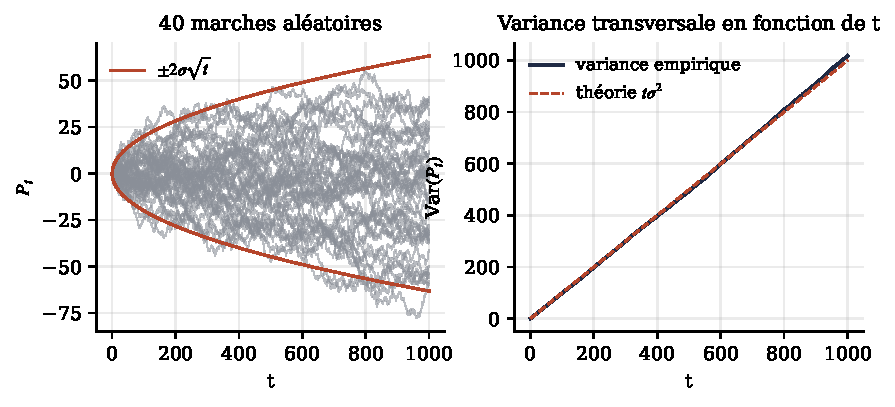
\includegraphics[width=0.92\textwidth]{ch01/h1_random_walk_variance.pdf}
\caption{À gauche, 40 marches aléatoires et l'enveloppe $\pm 2\sigma\sqrt{t}$. À droite, la variance transversale mesurée sur 20\,000 trajectoires suit la droite théorique $t\sigma^2$.}
\label{c1:fig:h1}
\end{figure}

\subsection{Prix, log-prix et rendements}
En pratique on modélise plutôt le \emph{logarithme} du prix comme une marche aléatoire (éventuellement avec une dérive $c$) : $\log P_t = c + \log P_{t-1} + \varepsilon_t$. Le rendement logarithmique $r_t = \log P_t - \log P_{t-1} = c + \varepsilon_t$ est alors un bruit blanc décalé, donc stationnaire. C'est pourquoi les économètres disent qu'un prix est \og intégré d'ordre 1\fg, noté $I(1)$ : il faut le différencier une fois pour obtenir une série stationnaire, notée $I(0)$. Cette notation sera formalisée au chapitre~4.

% =====================================================================
\section{Le processus autorégressif d'ordre un, AR(1)}
% =====================================================================

\subsection{Définition et résolution}

\begin{definition}
$(X_t)$ suit un AR(1) si $X_t = c + \varphi X_{t-1} + \varepsilon_t$, avec $(\varepsilon_t)$ bruit blanc de variance $\sigma^2$ et $c$, $\varphi$ deux constantes.
\end{definition}

On cherche d'abord le niveau $\mu$ autour duquel le processus pourrait se stabiliser. Si la série était constante égale à $\mu$ en l'absence de choc, on aurait $\mu = c + \varphi\mu$, donc, pour $\varphi \ne 1$,
\[
\mu = \frac{c}{1-\varphi}.
\]
En remplaçant $c = \mu(1-\varphi)$ dans la définition, on obtient la forme \og centrée\fg{}, beaucoup plus parlante :
\begin{equation}\label{c1:eq:ar1c}
X_t - \mu = \varphi\,(X_{t-1}-\mu) + \varepsilon_t.
\end{equation}
Notons $Y_t = X_t - \mu$ l'écart à la moyenne. Alors $Y_t = \varphi Y_{t-1} + \varepsilon_t$, et en remplaçant de proche en proche :
\begin{align*}
Y_t &= \varphi Y_{t-1} + \varepsilon_t = \varphi(\varphi Y_{t-2} + \varepsilon_{t-1}) + \varepsilon_t = \varphi^2 Y_{t-2} + \varphi\varepsilon_{t-1} + \varepsilon_t\\
&= \dots = \varphi^t Y_0 + \sum_{j=0}^{t-1}\varphi^j\,\varepsilon_{t-j}. \tag{$\ast$}
\end{align*}
La formule $(\ast)$ dit tout : l'écart d'aujourd'hui est l'écart initial multiplié par $\varphi^t$, plus une somme de chocs passés dont l'influence décroît géométriquement avec leur ancienneté (le choc d'il y a $j$ périodes pèse $\varphi^j$).

\subsection{Condition de stationnarité et moments}

\begin{proposition}\label{c1:prop:ar1}
Si $|\varphi| < 1$, l'AR(1) admet une solution stationnaire de moyenne $\mu = c/(1-\varphi)$, de variance et d'autocorrélation
\[
\gamma(0) = \frac{\sigma^2}{1-\varphi^2}, \qquad \rho(h) = \varphi^{h}\quad (h\ge0).
\]
Si $\varphi = 1$, le processus est une marche aléatoire (avec dérive $c$) et n'est pas stationnaire.
\end{proposition}
\begin{proof}
\emph{Moyenne.} Si $X$ est stationnaire, $\E X_t = \E X_{t-1} = m$. En prenant l'espérance dans la définition : $m = c + \varphi m$, donc $m = c/(1-\varphi) = \mu$.

\emph{Variance.} Dans \eqref{c1:eq:ar1c}, $\varepsilon_t$ est non corrélé avec $X_{t-1}$ (qui ne dépend que des chocs passés). Par la proposition~\ref{c1:prop:varspread} appliquée avec une covariance nulle : $\Var(X_t) = \varphi^2\Var(X_{t-1}) + \sigma^2$. Si la variance est constante, égale à $v$, alors $v = \varphi^2 v + \sigma^2$, soit $v(1-\varphi^2) = \sigma^2$ et $v = \sigma^2/(1-\varphi^2)$. Cette quantité n'est positive et finie que si $\varphi^2<1$, c'est-à-dire $|\varphi|<1$.

\emph{Autocovariance.} Avec $Y_t = X_t-\mu$, on itère $(\ast)$ sur $h$ pas à partir de $t-h$ : $Y_t = \varphi^h Y_{t-h} + \sum_{j=0}^{h-1}\varphi^j\varepsilon_{t-j}$. Les chocs $\varepsilon_{t-h+1},\dots,\varepsilon_t$ sont non corrélés avec $Y_{t-h}$, donc
\[
\gamma(h) = \Cov(Y_t, Y_{t-h}) = \varphi^h\Var(Y_{t-h}) = \varphi^h\gamma(0), \qquad \rho(h) = \frac{\gamma(h)}{\gamma(0)} = \varphi^h.
\]
\emph{Cas $\varphi=1$.} La définition devient $X_t = c + X_{t-1} + \varepsilon_t$ : c'est une marche aléatoire avec dérive, de variance croissante (proposition~\ref{c1:prop:rw}).
\end{proof}

\subsection{L'écriture \og retour à la moyenne\fg}

On soustrait $X_{t-1}-\mu$ des deux côtés de \eqref{c1:eq:ar1c} :
\begin{equation}\label{c1:eq:ecm}
\underbrace{X_t - X_{t-1}}_{\Delta X_t} = -\underbrace{(1-\varphi)}_{\kappa}\,(X_{t-1}-\mu) + \varepsilon_t.
\end{equation}
Avec $0<\varphi<1$, le coefficient $\kappa = 1-\varphi$ est compris entre 0 et 1 : à chaque période, le processus corrige en moyenne la fraction $\kappa$ de son écart à la moyenne. Si $X_{t-1}$ est au-dessus de $\mu$, la variation attendue est négative ; s'il est en dessous, elle est positive.

\begin{intuition}
Imaginez une balle attachée à un élastique fixé au point $\mu$. À chaque instant, quelqu'un la pousse au hasard (le choc $\varepsilon_t$), mais l'élastique la tire vers $\mu$ avec une force proportionnelle à la distance. Plus $\kappa$ est grand, plus l'élastique est raide. Avec $\varphi = 1$, il n'y a plus d'élastique : on retrouve le promeneur ivre. L'équation \eqref{c1:eq:ecm} préfigure le modèle à correction d'erreur du chapitre~4 et le processus d'Ornstein-Uhlenbeck du chapitre~5, qui en est la version en temps continu.
\end{intuition}

\subsection{La demi-vie}

\begin{proposition}[Demi-vie]\label{c1:prop:hl}
Pour $0<\varphi<1$, l'écart \emph{espéré} à la moyenne est divisé par deux en
\[
h_{1/2} = -\frac{\ln 2}{\ln\varphi} \quad\text{périodes},\qquad\text{avec l'approximation}\qquad h_{1/2} \approx \frac{\ln 2}{1-\varphi}\ \text{ quand } \varphi \text{ est proche de } 1.
\]
\end{proposition}
\begin{proof}
D'après $(\ast)$ appliquée à partir de la date $t$, $Y_{t+h} = \varphi^hY_t + \sum_{j=0}^{h-1}\varphi^j\varepsilon_{t+h-j}$. Les chocs futurs ont une espérance nulle, donc $\E[Y_{t+h}\mid Y_t] = \varphi^h Y_t$. On cherche $h$ tel que $\varphi^h = 1/2$. En prenant le logarithme : $h\ln\varphi = \ln(1/2) = -\ln 2$, d'où $h = -\ln 2/\ln\varphi$ (positif puisque $\ln\varphi<0$). Pour l'approximation, on pose $\varphi = 1-\kappa$ avec $\kappa$ petit ; le développement limité $\ln(1-\kappa) = -\kappa - \kappa^2/2 - \dots \approx -\kappa$ donne $h \approx \ln 2/\kappa$.
\end{proof}

\begin{table}[h]
\centering\small
\caption{Demi-vie en fonction de $\varphi$ (en nombre de périodes, par exemple en jours sur données quotidiennes).}
\label{c1:tab:hl}
\begin{tabular}{lccccc}
\toprule
$\varphi$ & 0,50 & 0,80 & 0,90 & 0,95 & 0,99 \\
\midrule
$h_{1/2}$ exacte $= -\ln2/\ln\varphi$ & 1,00 & 3,11 & 6,58 & 13,51 & 68,97 \\
approximation $\ln 2/(1-\varphi)$ & 1,39 & 3,47 & 6,93 & 13,86 & 69,31 \\
\bottomrule
\end{tabular}
\end{table}

\paragraph{Lecture pour le trading.} La demi-vie donne l'échelle de temps d'une stratégie. Une demi-vie de 6 jours signifie qu'un écart ouvert met typiquement une à deux semaines à se refermer ; une demi-vie de 70 jours immobilise le capital pendant des mois et multiplie les occasions de rupture. \citet{chan2013} recommande d'utiliser la demi-vie pour régler à la fois la fenêtre de calcul de la moyenne mobile et la durée de détention attendue.

\subsection{Vérification (H2)}

\begin{codebox}[ — script \texttt{h2\_ar1\_half\_life.py}]
\textbf{Hypothèses :} pour $\varphi = 0{,}95$ et $\sigma = 1$ : (a) $\gamma(0) = 1/(1-0{,}95^2) = 10{,}256$ ; (b) $\rho(h) = 0{,}95^h$ ; (c) demi-vie $13{,}51$ ; (d) biais de l'estimateur sur échantillon court.

\textbf{Résultats :} (a) variance mesurée sur 200\,000 points : $10{,}355$ ; (b) autocorrélation au retard 10 : $0{,}602$ contre $0{,}599$ en théorie ; (c) sur 20\,000 trajectoires partant d'un écart de 10, l'écart moyen passe sous 5 après $13{,}59$ périodes ; (d) voir le tableau~\ref{c1:tab:bias}.
\end{codebox}

\begin{table}[h]
\centering\small
\caption{Estimation de $\varphi$ et de la demi-vie par moindres carrés sur 2\,000 échantillons simulés ($\varphi = 0{,}95$, vraie demi-vie $13{,}51$).}
\label{c1:tab:bias}
\begin{tabular}{rccccc}
\toprule
Taille $n$ & $\overline{\hat\varphi}$ & biais & demi-vie médiane & quantile 5\,\% & quantile 95\,\% \\
\midrule
250 & 0,9343 & $-0{,}0157$ & 10,82 & 5,87 & 21,38 \\
1\,000 & 0,9460 & $-0{,}0040$ & 12,65 & 9,28 & 17,81 \\
5\,000 & 0,9493 & $-0{,}0007$ & 13,39 & 11,51 & 15,55 \\
\bottomrule
\end{tabular}
\end{table}

\begin{figure}[h]
\centering
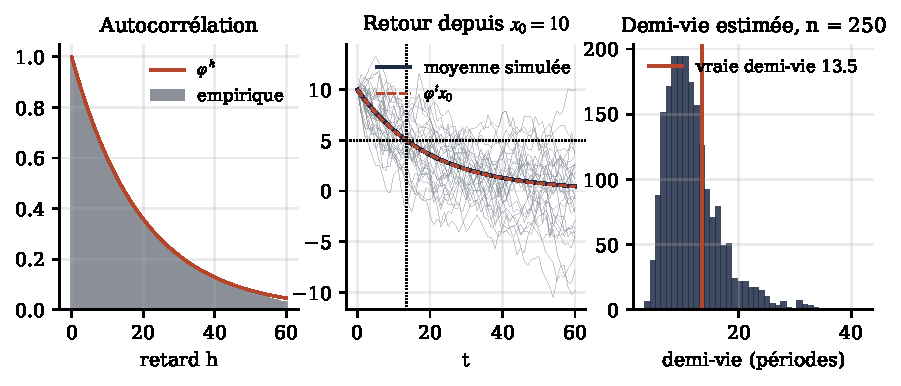
\includegraphics[width=0.98\textwidth]{ch01/h2_ar1_half_life.pdf}
\caption{À gauche, l'autocorrélation empirique suit $\varphi^h$. Au centre, 30 trajectoires partant de $x_0 = 10$ et leur moyenne, qui suit $\varphi^t x_0$ et coupe le niveau 5 à la demi-vie. À droite, la dispersion de la demi-vie estimée sur 250 observations (environ un an de données quotidiennes).}
\label{c1:fig:h2}
\end{figure}

\begin{pitfall}
Avec un an de données quotidiennes ($n = 250$), la demi-vie estimée est en médiane de 10,8 jours au lieu de 13,5, et dans 10\,\% des cas elle sort de l'intervalle $[5{,}9\,;\,21{,}4]$. L'estimateur de $\varphi$ est biaisé vers le bas ; l'approximation classique de \citet{kendall1954}, $\E[\hat\varphi]-\varphi \approx -(1+3\varphi)/n$, prédit $-3{,}85/250 = -0{,}0154$, très proche du biais mesuré ($-0{,}0157$). Conséquence pratique : sur historique court, une paire paraît revenir \emph{plus vite} qu'en réalité, ce qui pousse à trader trop souvent et à sous-estimer la durée de détention. Le chapitre~2 revient sur ce biais et le chapitre~5 sur l'estimation par maximum de vraisemblance.
\end{pitfall}

% =====================================================================
\section{De deux prix non stationnaires à un écart stationnaire}\label{c1:sec:coint}
% =====================================================================

\subsection{L'ivrogne et son chien}

\citet{murray1994} propose l'image suivante. Une promeneuse ivre sort du bar et erre au hasard : sa position est une marche aléatoire. Son chien, en laisse, erre lui aussi. Prise isolément, la trajectoire de chacun est imprévisible. Mais la laisse impose que la distance entre les deux reste bornée : quand le chien s'éloigne trop, la promeneuse l'appelle, ou le chien revient de lui-même. La \emph{distance} entre eux est stationnaire, alors que leurs \emph{positions} ne le sont pas.

\begin{definition}[Cointégration, version intuitive]
Deux séries $X_t$ et $Y_t$ non stationnaires de type $I(1)$ sont \emph{cointégrées} s'il existe un nombre $\beta$ tel que l'écart $S_t = Y_t - \beta X_t$ soit stationnaire. Le vecteur $(1,-\beta)$ est appelé vecteur de cointégration. La définition formelle, les tests et les généralisations à plusieurs actifs sont l'objet du chapitre~4 \citep{englegranger1987,johansen1991}.
\end{definition}

Voilà l'idée fondatrice de l'arbitrage statistique par cointégration : on ne sait pas prédire $X$ ni $Y$, mais si $S$ est stationnaire, on sait que ses écarts à la moyenne sont temporaires, et la section précédente nous dit à quelle vitesse ils se résorbent.

\subsection{Corrélation n'est pas cointégration}

C'est l'erreur la plus fréquente chez les débutants : choisir des paires parce que leurs rendements sont fortement corrélés. La corrélation des rendements mesure si les deux actifs bougent \emph{dans le même sens le même jour}. La cointégration mesure si leurs \emph{niveaux} restent liés \emph{à long terme}. Les deux propriétés sont logiquement indépendantes.

\begin{example}[Deux paires construites pour le montrer]
\textbf{Paire A} : $X$ et $Y$ sont deux marches aléatoires dont les chocs quotidiens sont corrélés à $0{,}9$. Elles bougent presque toujours ensemble, mais rien ne ramène l'une vers l'autre : leur écart est lui-même une marche aléatoire.

\textbf{Paire B} : $X$ est une marche aléatoire et $Y_t = X_t + s_t$, où $s_t$ est un AR(1) avec $\varphi = 0{,}5$ et des chocs d'écart-type $\sigma_s = 2$, plus grand que celui des chocs de $X$ (égal à 1). L'écart $Y - X = s$ est stationnaire, mais les rendements de $Y$ sont dominés par le bruit de $s$.
\end{example}

On peut même calculer la corrélation des rendements de la paire B. Les rendements sont $\Delta X_t = u_t$ et $\Delta Y_t = u_t + \Delta s_t$. Calculons d'abord la variance de $\Delta s_t = s_t - s_{t-1}$ par la proposition~\ref{c1:prop:varspread} (avec $\beta = 1$) et la proposition~\ref{c1:prop:ar1} :
\[
\Var(\Delta s_t) = \gamma(0) + \gamma(0) - 2\gamma(1) = 2\gamma(0)(1-\varphi), \qquad \gamma(0) = \frac{\sigma_s^2}{1-\varphi^2} = \frac{4}{0{,}75} = 5{,}33,
\]
donc $\Var(\Delta s_t) = 2\times 5{,}33\times 0{,}5 = 5{,}33$. Comme $u_t$ est indépendant de $s$, $\Cov(\Delta X_t,\Delta Y_t) = \Var(u_t) = 1$ et $\Var(\Delta Y_t) = 1 + 5{,}33 = 6{,}33$. D'où
\[
\Corr(\Delta X_t,\Delta Y_t) = \frac{1}{\sqrt{1}\sqrt{6{,}33}} \approx 0{,}397.
\]

\begin{codebox}[ — script \texttt{h3\_correlation\_vs\_cointegration.py}]
\textbf{Hypothèse :} forte corrélation des rendements sans cointégration (A) et faible corrélation avec cointégration (B) sont possibles. \textbf{Protocole :} 1\,000 jours par paire ; test ADF sur l'écart $Y-X$ (utilisé ici comme boîte noire, il sera étudié au chapitre~3) ; 500 répétitions. \textbf{Résultats :} paire A : corrélation moyenne des rendements $0{,}90$, le test conclut à la stationnarité de l'écart dans seulement $5{,}8\,\%$ des cas, ce qui correspond au taux de fausses alertes attendu d'un test à 5\,\%. Paire B : corrélation moyenne $0{,}395$ (le calcul théorique donnait $0{,}397$), et le test conclut à la stationnarité dans $100\,\%$ des cas.
\end{codebox}

\begin{figure}[h]
\centering
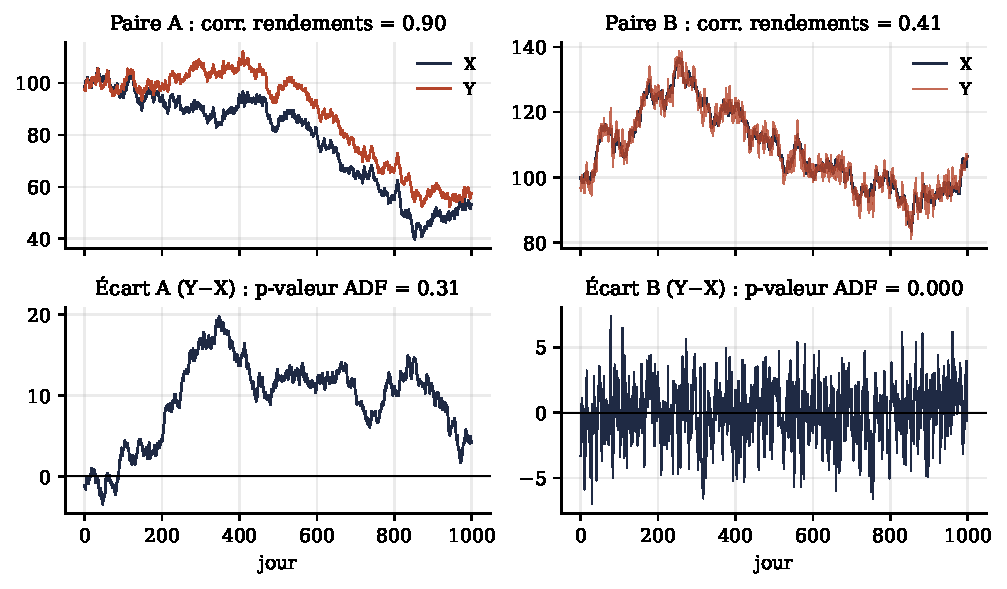
\includegraphics[width=0.9\textwidth]{ch01/h3_correlation_vs_cointegration.pdf}
\caption{En haut, les prix des deux paires ; en bas, leurs écarts. La paire A, très corrélée, dérive sans retour ; la paire B, peu corrélée, a un écart qui oscille autour de zéro.}
\label{c1:fig:h3}
\end{figure}

\subsection{Le piège de la régression fallacieuse}\label{c1:sec:spurious}

Si l'on régresse un prix sur un autre pour trouver $\beta$, on risque de \og découvrir\fg{} une relation qui n'existe pas. \citet{granger1974} ont montré que la régression d'une marche aléatoire sur une autre, \emph{indépendante}, produit très souvent une pente \og significative\fg{} au sens du test de Student usuel et un $R^2$ élevé. La raison : les deux séries ont des tendances aléatoires qui, sur un échantillon fini, semblent aller dans le même sens ou en sens opposé, et les hypothèses du test de Student (résidus non corrélés et stationnaires) sont violées.

\begin{codebox}[ — script \texttt{h4\_spurious\_regression.py}]
\textbf{Hypothèse :} régresser deux marches aléatoires indépendantes rejette \og pente nulle\fg{} bien plus souvent que 5\,\%. \textbf{Protocole :} 2\,000 répétitions, $n = 500$. \textbf{Résultats :} régression en niveaux : la pente est déclarée significative à 5\,\% dans $89\,\%$ des cas, le $R^2$ médian vaut $0{,}17$ et dépasse $0{,}3$ dans $35\,\%$ des cas. Régression des rendements : $4{,}3\,\%$ de rejets, conforme aux 5\,\% attendus, et $R^2$ médian de $0{,}0009$.
\end{codebox}

\begin{figure}[h]
\centering
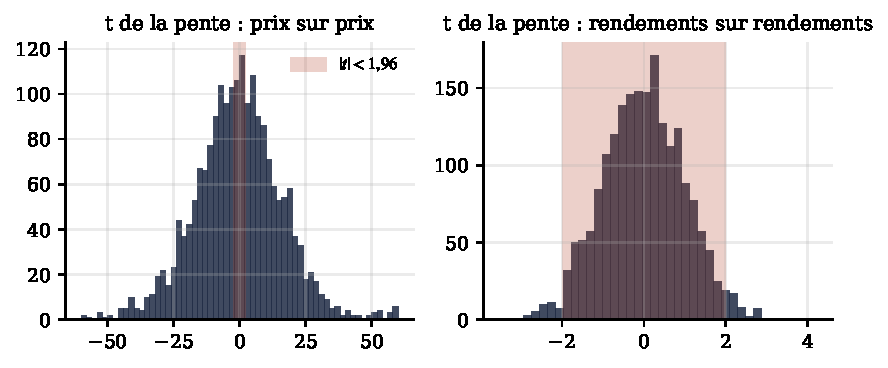
\includegraphics[width=0.85\textwidth]{ch01/h4_spurious_regression.pdf}
\caption{Distribution de la statistique $t$ de la pente. En niveaux (gauche), elle est très dispersée et sort presque toujours de la zone $|t|<1{,}96$ ; en rendements (droite), elle suit à peu près une loi normale centrée réduite.}
\label{c1:fig:h4}
\end{figure}

\begin{pitfall}
Une régression de prix sur prix ne prouve rien par elle-même. Elle n'a de sens que si l'on vérifie ensuite que les \emph{résidus} sont stationnaires : c'est exactement la méthode d'Engle et Granger, qui utilise des valeurs critiques spécifiques justement parce que les tests usuels sont faussés dans ce contexte (chapitre~4).
\end{pitfall}

% =====================================================================
\section{Du spread au signal : une première règle de trading}
% =====================================================================

\subsection{Construction sans information future}

On dispose de deux séries de prix $X_t$ et $Y_t$. On coupe l'historique en deux : une \emph{période de formation} (les $n_f$ premières dates) et une \emph{période de trading} (les suivantes). Tout ce qui est estimé l'est \emph{uniquement} sur la formation.
\begin{enumerate}
\item Sur la formation, on estime $Y_t = \alpha + \beta X_t + e_t$ par moindres carrés (proposition~\ref{c1:prop:hedge}), d'où $\hat\alpha$, $\hat\beta$, puis la moyenne $m$ et l'écart-type $d$ des résidus.
\item Sur la période de trading, on calcule l'écart $S_t = Y_t - \hat\beta X_t - \hat\alpha$ et le \emph{z-score} $z_t = (S_t - m)/d$.
\item Règle : si l'on n'a pas de position et $z_t > 2$, on \emph{vend} l'écart (on vend une unité de $Y$ et on achète $\hat\beta$ unités de $X$) ; si $z_t < -2$, on \emph{achète} l'écart ; on sort quand $z_t$ repasse par 0.
\end{enumerate}

\subsection{Comptabilité du gain et des coûts}

Notons $q_t \in \{-1, 0, +1\}$ la position en écart décidée à la clôture de la date $t$. Le gain de la date $t$ à la date $t+1$ est
\[
\text{G}_{t+1} = q_t\,(S_{t+1} - S_t).
\]
Le décalage d'indice est essentiel : la position décidée avec l'information de la date $t$ s'applique à la variation \emph{suivante}. Écrire $q_{t+1}(S_{t+1}-S_t)$ reviendrait à utiliser le prix de demain pour décider aujourd'hui, l'erreur d'anticipation (\emph{look-ahead bias}) la plus fréquente dans les \emph{backtests} amateurs. À chaque changement de position, on paie un coût proportionnel au notionnel échangé sur les deux jambes :
\[
\text{coût}_t = c\;|q_t - q_{t-1}|\;\big(Y_t + |\hat\beta|X_t\big),
\]
où $c$ est exprimé en fraction (5 pb $= 0{,}0005$).

\subsection{Test dans un monde simulé (H5)}

Pour isoler l'effet de chaque ingrédient, on teste la règle dans un monde où la vérité est connue : $X$ est une marche aléatoire autour de 100, $Y_t = 1{,}5\,X_t + s_t$ et $s_t$ est un AR(1) avec $\varphi = 0{,}9$ (demi-vie de 6,6 jours) et des chocs d'écart-type 1. La formation dure 500 jours, le trading 1\,000 jours, et l'on répète l'expérience 400 fois.

\begin{codebox}[ — script \texttt{h5\_zscore\_toy\_strategy.py}]
\textbf{Estimation :} $\hat\beta$ vaut en moyenne $1{,}4999$ (écart-type $0{,}058$) : la régression retrouve bien le vrai ratio \emph{quand la paire est réellement cointégrée}. \textbf{Gain et coûts :} voir le tableau~\ref{c1:tab:h5}. \textbf{Rupture :} dans une seconde série de mondes, l'écart devient une marche aléatoire ($\varphi = 1$) au 200\textsuperscript{e} jour de trading ; on compare les résultats réalisés \emph{après} ce jour (tableau~\ref{c1:tab:h5b}).
\end{codebox}

\begin{table}[h]
\centering\small
\caption{Règle $|z|>2$, sortie à $z = 0$, relation stable. Moyennes sur 400 mondes simulés ; gain exprimé en dollars pour une unité d'écart.}
\label{c1:tab:h5}
\begin{tabular}{rcccc}
\toprule
Coût par jambe & Gain moyen & Part des mondes gagnants & Sharpe annualisé médian & Allers-retours \\
\midrule
0 pb & 70,25 & 100\,\% & 2,02 & 13,3 \\
5 pb & 66,21 & 100\,\% & 1,91 & 13,3 \\
10 pb & 62,17 & 100\,\% & 1,80 & 13,3 \\
25 pb & 50,06 & 100\,\% & 1,45 & 13,3 \\
50 pb & 29,88 & 98,8\,\% & 0,84 & 13,3 \\
\bottomrule
\end{tabular}
\end{table}

\begin{table}[h]
\centering\small
\caption{Après le 200\textsuperscript{e} jour de trading, coût de 5 pb par jambe : relation stable contre relation rompue.}
\label{c1:tab:h5b}
\begin{tabular}{lcc}
\toprule
 & Relation stable & Relation rompue \\
\midrule
Gain moyen par monde & 53,41 & $-2{,}09$ (erreur-type 1,27) \\
Quantile 5\,\% du gain & 27,64 & $-46{,}66$ \\
Part des trades gagnants & 99,1\,\% & 78,0\,\% \\
Gain moyen d'un trade gagnant & 5,01 & 5,17 \\
Perte moyenne d'un trade perdant & $-1{,}73$ & $-20{,}40$ \\
Pire trade & $-5{,}57$ & $-83{,}76$ \\
\bottomrule
\end{tabular}
\end{table}

\begin{figure}[h]
\centering
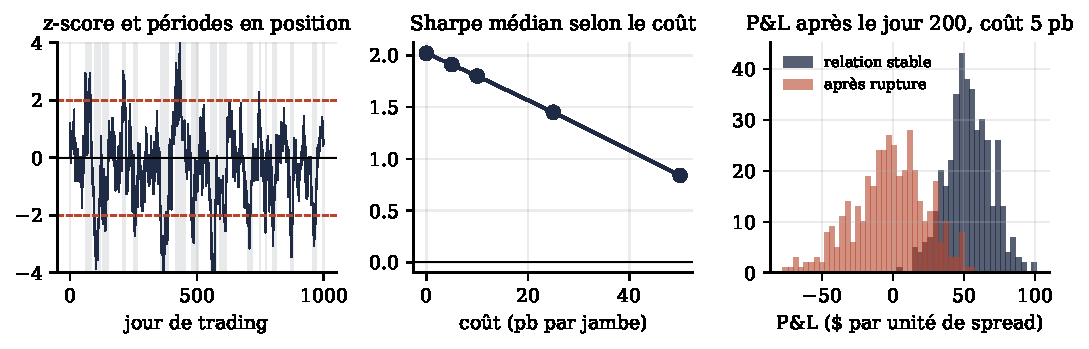
\includegraphics[width=0.98\textwidth]{ch01/h5_zscore_toy_strategy.pdf}
\caption{À gauche, le \emph{z-score} d'un monde simulé, les seuils $\pm 2$ et les périodes en position (grisées). Au centre, le Sharpe médian baisse avec le coût. À droite, distribution du gain réalisé après le 200\textsuperscript{e} jour, avec et sans rupture.}
\label{c1:fig:h5}
\end{figure}

\needspace{8\baselineskip}
\paragraph{Ce que montrent les chiffres.}
\begin{enumerate}
\item \emph{Quand l'écart est réellement stationnaire, la règle gagne.} Chaque aller-retour capture environ deux écarts-types de l'écart ($2\times\sqrt{1/(1-0{,}81)} \approx 4{,}6$), ce qui correspond au gain moyen par trade d'environ 5.
\item \emph{Les coûts mordent vite.} Un aller-retour échange quatre fois un notionnel d'environ 150 (deux jambes, entrée et sortie), soit environ 600 ; à 5 pb, cela coûte $0{,}30$ par aller-retour, ce qui explique la baisse de $70{,}25$ à $66{,}21$ sur 13,3 allers-retours. À 50 pb, le Sharpe est divisé par plus de deux.
\item \emph{Un fort taux de réussite ne prouve rien.} Après la rupture, 78\,\% des trades restent gagnants, mais la perte moyenne d'un trade perdant ($-20{,}4$) est quatre fois le gain moyen d'un trade gagnant, et le gain total moyen devient statistiquement indiscernable de zéro (moins les coûts). C'est le profil \og ramasser des pièces devant un rouleau compresseur\fg{} : une règle de retour à la moyenne sans contrôle de rupture continue d'accumuler une position perdante en attendant un retour qui ne vient plus.
\end{enumerate}

\begin{pitfall}
Ces résultats proviennent d'un monde simulé \emph{construit pour que la stratégie fonctionne} : écart parfaitement stationnaire, paramètres constants, chocs gaussiens, exécution au prix de clôture, pas de coût d'emprunt des titres vendus à découvert. Sur données réelles, chacun de ces points dégrade la performance. Le monde simulé sert à mesurer l'effet d'un ingrédient à la fois ; il ne prédit pas la rentabilité d'une paire réelle.
\end{pitfall}

% =====================================================================
\section{Ce que la théorie apporte, et ses limites}
% =====================================================================

\paragraph{Ce qu'elle apporte.} Un langage précis : on ne dit plus \og ces deux actions se ressemblent\fg, mais \og l'écart est-il stationnaire, avec quelle demi-vie et quelle variance ?\fg. Des ordres de grandeur avant tout \emph{backtest} : la variance minimale d'un écart ($\sigma_Y^2(1-\rho^2)$), le gain par aller-retour ($\approx$ deux écarts-types de l'écart) et le coût par aller-retour se calculent à la main et disent tout de suite si une idée a une chance de survivre aux frais. Des tests pour éviter les illusions statistiques les plus courantes (régression fallacieuse, corrélation confondue avec cointégration).

\paragraph{Ses limites.}
\begin{itemize}
\item \textbf{La stationnarité ne se démontre jamais sur données.} Un test peut seulement dire que les données sont compatibles avec elle, et sur des échantillons courts la puissance des tests est faible (chapitre~3).
\item \textbf{Les paramètres changent.} $\beta$, $\varphi$ et $\sigma$ dérivent avec les régimes de marché ; une relation solide pendant cinq ans peut se rompre en une semaine (fusion, changement de modèle économique, choc réglementaire). Les chapitres~8 (Kalman) et~17 (détection de rupture) y répondent en partie.
\item \textbf{Les chocs ne sont pas gaussiens.} Les rendements financiers ont des queues épaisses : un écart à $4\sigma$ est beaucoup plus fréquent que $0{,}006\,\%$ du temps. Les seuils fondés sur la loi normale sous-estiment le risque extrême.
\item \textbf{Les frictions ne sont pas modélisées.} Fourchette achat-vente, impact, coût d'emprunt des titres, financement des positions, latence et exécution partielle sont traités dans la partie~III.
\item \textbf{La recherche de paires crée des faux positifs.} Tester 1\,000 paires au seuil de 5\,\% produit en moyenne 50 \og paires cointégrées\fg{} par pur hasard (chapitre~16).
\end{itemize}

% =====================================================================
\section{Fiche à recopier au tableau blanc}
% =====================================================================

\begin{whiteboard}
\begin{itemize}[leftmargin=1.2em]
\item \textbf{Arbitrage pur :} coût $\le 0$, perte impossible, gain possible. \textbf{Statistique :} $v(0)=0$, $\E[v(t)]\to>0$, $\Prob(v(t)<0)\to0$, $\Var(v(t))/t\to0$.
\item \textbf{Variance d'un écart :} $\Var(Y-\beta X) = \sigma_Y^2 + \beta^2\sigma_X^2 - 2\beta\Cov(X,Y)$.
\item \textbf{Couverture optimale :} $\beta^\star = \Cov(X,Y)/\sigma_X^2 = \rho\,\sigma_Y/\sigma_X$ ; variance restante $\sigma_Y^2(1-\rho^2)$.
\item \textbf{Stationnarité faible :} $\E X_t = \mu$, $\Var X_t = \gamma(0)$, $\Cov(X_t,X_{t-h}) = \gamma(h)$, indépendants de $t$.
\item \textbf{Marche aléatoire :} $P_t = P_0 + \sum\varepsilon_i$ ; $\E P_t = P_0$ ; $\Var P_t = t\sigma^2$ ; non stationnaire ; $I(1)$.
\item \textbf{AR(1) :} $X_t - \mu = \varphi(X_{t-1}-\mu) + \varepsilon_t$ ; stationnaire si $|\varphi|<1$ ; $\mu = c/(1-\varphi)$ ; $\gamma(0) = \sigma^2/(1-\varphi^2)$ ; $\rho(h) = \varphi^h$.
\item \textbf{Retour à la moyenne :} $\Delta X_t = -(1-\varphi)(X_{t-1}-\mu) + \varepsilon_t$.
\item \textbf{Demi-vie :} $h_{1/2} = -\ln2/\ln\varphi \approx \ln 2/(1-\varphi)$.
\item \textbf{Cointégration (intuition) :} $X, Y \sim I(1)$ et $Y - \beta X \sim I(0)$.
\item \textbf{Z-score :} $z_t = (S_t - m)/d$, avec $m$, $d$ estimés \emph{sur la formation seulement}.
\item \textbf{Gain sans anticipation :} $G_{t+1} = q_t(S_{t+1}-S_t)$.
\end{itemize}
\end{whiteboard}

% =====================================================================
\section{Exercices}
% =====================================================================

\begin{exercise}
Montrez que $\Var(aX + bY) = a^2\sigma_X^2 + b^2\sigma_Y^2 + 2ab\Cov(X,Y)$, puis retrouvez la proposition~\ref{c1:prop:varspread} comme cas particulier.
\end{exercise}

\begin{exercise}
Deux actifs ont des volatilités quotidiennes $\sigma_X = 1{,}2\,\%$ et $\sigma_Y = 1{,}5\,\%$ et une corrélation de $0{,}85$. Calculez $\beta^\star$ et la volatilité quotidienne de l'écart couvert. Quelle corrélation faudrait-il pour que cette volatilité tombe sous $0{,}3\,\%$ ?
\end{exercise}

\begin{exercise}
Sur données quotidiennes, on estime $\hat\varphi = 0{,}98$. Calculez la demi-vie exacte et approchée. Quel $\varphi$ correspond à une demi-vie de 10 jours ? En utilisant le tableau~\ref{c1:tab:bias}, discutez la fiabilité de cette estimation si elle repose sur un an de données.
\end{exercise}

\begin{exercise}
Montrez que l'AR(1) avec $\varphi = -0{,}5$ est stationnaire. Que vaut son autocorrélation aux retards 1, 2 et 3 ? Décrivez l'allure d'une trajectoire et ce que cela signifierait pour un trader.
\end{exercise}

\begin{exercise}
Démontrez que, pour une marche aléatoire, $\Corr(P_t,P_{t+h}) = \sqrt{t/(t+h)}$, et calculez cette corrélation pour $t = 250$ et $h = 5$. Pourquoi cette valeur proche de 1 n'indique-t-elle aucune prévisibilité exploitable ?
\end{exercise}

\begin{exercise}[à coder]
Modifiez \texttt{h5\_zscore\_toy\_strategy.py} pour tester des seuils d'entrée de 1 ; 1,5 ; 2 ; 2,5 et 3. Quel seuil donne le meilleur Sharpe à 5 pb ? Pourquoi serait-il dangereux de retenir ce seuil sur données réelles si on l'a choisi sur la même période que celle où on mesure la performance ? (Indice : chapitre~16.)
\end{exercise}

\begin{exercise}[à coder]
Ajoutez à \texttt{h5} un stop-loss : on ferme la position si $|z_t| > 4$. Mesurez son effet dans le monde stable et dans le monde avec rupture. Le stop-loss coûte-t-il quelque chose quand la relation est stable ?
\end{exercise}

\begin{exercise}[données réelles]
Téléchargez les prix quotidiens de deux ETF adossés à l'or (par exemple via Interactive Brokers). Estimez $\hat\beta$, l'écart, sa demi-vie, et appliquez le test ADF. S'agit-il d'arbitrage statistique ou de quasi-arbitrage au sens de la section~\ref{c1:sec:arb} ? Rapprochez votre réponse du moteur \texttt{atjte} (chapitre~0, section~\ref{c0:atjte}).
\end{exercise}

% =====================================================================
\section{Pour aller plus loin}
% =====================================================================

\begin{toread}
\begin{itemize}[leftmargin=1.2em]
\item \citet{hamilton1994}, chapitre~3, sections 3.1 (espérance, stationnarité, ergodicité), 3.2 (bruit blanc) et 3.4 (processus autorégressifs) : la référence pour les démonstrations de la section~6.
\item \citet{tsay2010}, chapitre~2, sections sur la stationnarité, l'autocorrélation, le bruit blanc et les modèles AR simples : même contenu, orienté données financières, avec des exemples.
\item \citet{chan2013}, chapitre~2 (\og The Basics of Mean Reversion\fg) : stationnarité, demi-vie et cointégration vues par un praticien, avec code.
\item \citet{murray1994} : trois pages, l'image de l'ivrogne et du chien ; à lire en entier.
\item \citet{hogan2004} : la section qui définit l'arbitrage statistique (définition~\ref{c1:def:statarb} de ce chapitre).
\item \citet{granger1974} : l'article original sur la régression fallacieuse, court et lisible.
\item Chapitre~0, section~\ref{c0:litt} : la revue de littérature, pour situer la suite.
\end{itemize}
\end{toread}

\paragraph{Prochain chapitre.} Le chapitre~2 dérive les moindres carrés sous forme matricielle, explique pourquoi régresser $Y$ sur $X$ ne donne pas le même ratio que régresser $X$ sur $Y$, introduit le maximum de vraisemblance et revient sur le biais de petit échantillon mesuré au tableau~\ref{c1:tab:bias}.

\section{Scripts du chapitre}

\begin{center}\small
\begin{tabular}{ll}
\toprule
Élément & Script (\texttt{code/ch01/}) \\
\midrule
Figure~\ref{c1:fig:h1} & \texttt{h1\_random\_walk\_variance.py} \\
Figure~\ref{c1:fig:h2}, tableau~\ref{c1:tab:bias} & \texttt{h2\_ar1\_half\_life.py} \\
Figure~\ref{c1:fig:h3} & \texttt{h3\_correlation\_vs\_cointegration.py} \\
Figure~\ref{c1:fig:h4} & \texttt{h4\_spurious\_regression.py} \\
Figure~\ref{c1:fig:h5}, tableaux~\ref{c1:tab:h5} et~\ref{c1:tab:h5b} & \texttt{h5\_zscore\_toy\_strategy.py} \\
\bottomrule
\end{tabular}
\end{center}

\noindent Chaque script écrit ses chiffres dans \texttt{code/ch01/results/} sous le même nom avec l'extension \texttt{.json}. Pour tout relancer : \texttt{cd code/ch01 \&\& for f in h*.py; do python \$f; done} (dépendances : \texttt{numpy}, \texttt{matplotlib}, \texttt{statsmodels}).

\subsection*{Estimer une demi-vie en quatre lignes}

\begin{lstlisting}[language=Python]
import numpy as np
def half_life(x):
    """Demi-vie (en periodes) estimee par MCO de x_t sur x_{t-1}."""
    b = np.polyfit(x[:-1], x[1:], 1)[0]     # pente = phi estime
    return -np.log(2) / np.log(b) if 0 < b < 1 else np.inf
\end{lstlisting}

